\documentclass{article}
\usepackage[margin=1.5cm]{geometry}
\usepackage[us]{tkz-fn}
\begin{document}
\tkzFnDef{f}{1/((1e9*x/11.778)*3.273e-8-3.273e-8+1)}
\begin{tikzpicture}[scale=.75]
  \tkzFnInit[xmin=0,xmax=6,ymin=0,ymax=1,ystep=.2]
  \tkzFnAxes[box]
  \tkzFnDraw[blue,mark=*,mark size=1.5pt,samples=13,domain=0:5](f)
  \tkzFnDrawData[red,mark=square*,mark size=1.5pt]{.125/.744}
\end{tikzpicture}
\begin{tikzpicture}[scale=.75]
  \tkzFnInit[xmin=0,xmax=6,ymin=0,ymax=1,ystep=.2]
  \tkzFnAxes[box]
  \tkzFnDraw[blue,mark=*,mark size=1.5pt,samples=25](f)
  \tkzFnDrawData[red,mark=square*,mark size=1.5pt]{.125/.744}
\end{tikzpicture}
\begin{tikzpicture}[scale=.75]
  \tkzFnInit[xmin=0,xmax=6,ymin=0,ymax=1,ystep=.2,enlarge]
  \tkzFnAxes[box,xlabel=$x$,ylabel={$f(x)$}]
  \tkzFnDraw[blue,mark=*,mark size=1.5pt,samples=25](f)
  \tkzFnDrawData[red,mark=square*,mark size=1.5pt]{.125/.744}
\end{tikzpicture}

\tkzFnSetup{axes=box,format=fr}
\begin{tikzpicture}[scale=.6]
  \tkzFnInit[xmin=-3,xmax=3,ymin=0,ymax=20000,ystep=4000]
  \tkzFnGrid
  \tkzFnAxes[xlabel=$t$,ylabel=Population]
  \tkzFnDraw[red,thick,smooth,samples=7]{2000*x^2}
\end{tikzpicture}
\begin{tikzpicture}[scale=.6]
  \tkzFnInit[xmin=-7,xmax=7,ymin=-1,ymax=1,ystep=.5]
  \tkzFnAxes[trig=2]
  \tkzFnDraw{sin(x)}
\end{tikzpicture}
\tkzFnSetup{axes=school}
\begin{tikzpicture}[scale=.6]
  \tkzFnInit[xmin=-3,xmax=3,ymin=-1,ymax=3]
  \tkzFnAxes
  \tkzFnDraw{x^2/3}
\end{tikzpicture}
\end{document}
